\documentclass[12pt]{article}


\usepackage[english]{babel}
\usepackage[utf8]{inputenc}
\usepackage{amsmath}
\usepackage{bbm}
\usepackage{graphicx}
\usepackage{amsfonts}
\usepackage[colorinlistoftodos]{todonotes}

\graphicspath{ {images/} }

\title{CS 5876 - HW 3}

\author{Joshua Campbell (jac677) , Michael Wang (mzw4) , Neil Parker (nwp7) }

\date{\today}

\begin{document}
\maketitle

\begin{enumerate}

\item[Q1)]
	
	\begin{enumerate}
	\item[1)] The parameters of the model are:
		\begin{itemize}
		\item $\mu_1$ - The first red-apple tree location ($ \mu_1 \in \mathbb{R}^2 $)
		\item $\mu_2$ - The first green-apple tree location ($ \mu_2 \in \mathbb{R}^2 $)
		\item $\sigma$ - The parameter defining variance ($ \sigma^2 $) for both $ \mu_1 and \mu_2 $
		\item $\pi$ - A mixture distribution over the $ K=2 $ types of trees
		\end{itemize}
	
	\item[2)] There O(2N) nodes and $O(N^2)$ edges. Each time step is independent of others, in terms of selecting which type of tree to sprout. However, choosing the location depends on this choice as well as all the previous tree locations and previous tree type choices, since there is no indication (in this model) of which location was the most recent location of the corresponding tree choice. Thus, at each time step, the location at the time step will have one edge from the tree choice at that time test, and an edge from all the previous tree choices and tree locations.
	
	\item[3)] There are 7(N-1) edges in the model, where N is the number of iterations. The states looks like below. Each $X_t^i$ depends on $X_{t-1}^i$ and $C_t$. $X_t$ depends on $C_t$ to choose which value of $X_t^i$ to assume. Each $C_t$ is independent and thus does not depend on any of the variables.
		
	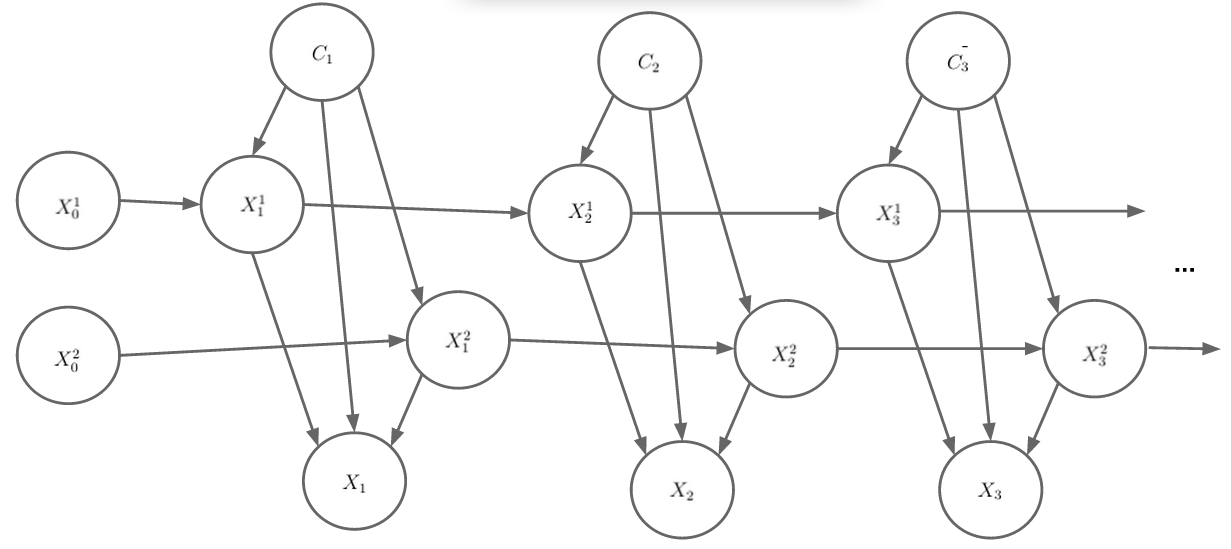
\includegraphics[width=0.75\textwidth]{Q1-3.png}
	
	\item[4)] $P(C_t = i | \text{parents}) = \pi$
	
	$P(X_t | C_t = i, X^1_{t}, X^2_{t}) = 1$
	
	$P(X^{(i)}_t | C_t, X^{(i)}_{t-1}) = \mathbbm{1}_{ i = C_t }N(X^{(i)}_{t-1}, \sigma^2 I)$ + $\mathbbm{1}_{ i \neq C_t} $
	
	$P(X^1_0) = N(\mu_1, \sigma^2 I)$
	
	$P(X^2_0) = N(\mu_2, \sigma^2 I)$
	
	\item[5)] For variable elimination (and also the order we will eliminate variables):

	Eliminate $X_0^1: m_{1, \theta}(X_0^1, X_1^1, C_1) =
		\int_{X_0^1}P(X_0^1)P(X_1^1 | C_1, X_0^1)$
	
	Eliminate $X_0^2: m_{2, \theta}(X_0^2, X_1^2, C_1) = 
		\int_{X_0^1}P(X_0^2)P(X_1^2 | C_1, X_0^2)$
	
	Eliminate  $X_1^1:  m_{3, \theta}(X_1^1, X_2^1, C_2, C_1) =
		\int_{X_1^1} P(X_1^1) P(X_2^1 | C_2, X_1^1) m_{1, \theta}$
		
	Eliminate  $X_1^2:  m_{4, \theta}(X_1^2, X_2^2, C_2, C_1) =
		\int_{X_1^2} P(X_1^2) P(X_2^2 | C_2, X_1^2) m_{2, \theta}$
		
	Eliminate  $X_2^1:  m_{5, \theta}(X_2^1, X_3^1, C_3, C_2, C_1) =
		\int_{X_2^1} P(X_2^1) P(X_3^1 | C_3, X_2^1) m_{3, \theta}$
		
	Eliminate  $X_2^2:  m_{6, \theta}(X_2^2, X_3^2, C_3, C_2, C_1) =
		\int_{X_2^2} P(X_2^2) P(X_3^2 | C_3, X_2^2) m_{4, \theta}$		
		
	Repeat for all $X^i_t$'s, defining up to $m_{2N+2, \theta}$.		
		
	Eliminate $C_1: k_{1, \theta}(C_1, C_2, C_3, ...) = 
		\sum_{C_1} m_{2N+2, \theta}$
		
	Eliminate $C_2: k_{2, \theta}(C_2, C_3, ...) = 
		\sum_{C_2} k_{1, \theta}$
		
	Eliminate $C_3: k_{3, \theta}(C_3, C_4, ...) = 
		\sum_{C_3} k_{2, \theta}$
		
	Repeat for all $C_t$'s, defining up to $k_{N-1, \theta}$
		
	Note that all $X_t$'s are deterministic.
	
	\end{enumerate}

\item[Q2)]

	\begin{enumerate}
	\item[1)] The hidden variables are the set \{$C_t$\}. The set of observed variables are the set \{$X_t$\}.
	
	\item[2)] $\log(P_\theta(O, H)) = \log \prod_{t=1}^N P(C_t) P(X_t | X_t^1, X_t^2, C_t$)$P(X^1_t | C_t, X^1_{t-1})P(X^2_t | C_t, X^2_{t-1})$
	$\log(P_\theta(O, H)) = \log \prod_{t=1}^N P(C_t)P(X^1_t | C_t, X^1_{t-1})P(X^2_t | C_t, X^2_{t-1})$
	
	= $\sum_{t=1}^N \{ log(P(C_t)) + log(P(X^1_t | C_t, X^1_{t-1})\} + log(P(X^2_t | C_t, X^2_{t-1})\}$
	
	\item[3)] 
	$\sum_H Q^i(H) log P_\theta(O,H) =$	
	
	$\sum_{t=1}^N \sum_{H} \{ Q^i(H)( log(P(C_t)) + log(P(X^1_t | C_t, X^1_{t-1})\} + log(P(X^2_t | C_t, X^2_{t-1})) \}$ 
	
	$ \\ $	
	
	$Q^i(H) = P(C_1=h, C_2=j, C_3=k, ...)$ 
	
	$= \prod_{t=1}^N P(C_i=j) = \prod_{t=1}^N Q^i_t(H_t)$
	
	$ \\ $	
	
	$Q^i_t(C_t =k) = P(C_t = k | X_t, \theta^{(i-1)}) =$
	
	$P(X_t | C_t = k, \theta^{(i-1)}) P(C_t = k | \theta^{(i-1)}) =
	P(C_t = k | \theta^{(i-1)})$
	
	$ \\ $	
	
	Thus,
	$\sum_H Q^i(H) log P_\theta(O,H) =$	
	
	$\sum_{t=1}^N \sum_{C_1,..,C_t} \{ P(C_1,...,C_t)( log(P(C_t)) + log(P(X^1_t | C_t, X^1_{t-1})\} + log(P(X^2_t | C_t, X^2_{t-1})) \}$ 
	\end{enumerate}

\end{enumerate}


\end{document}